
\hypertarget{working_app}{}
\section{Application options}
\index{application options}

\begin{figure}[h!]
  \begin{center}
    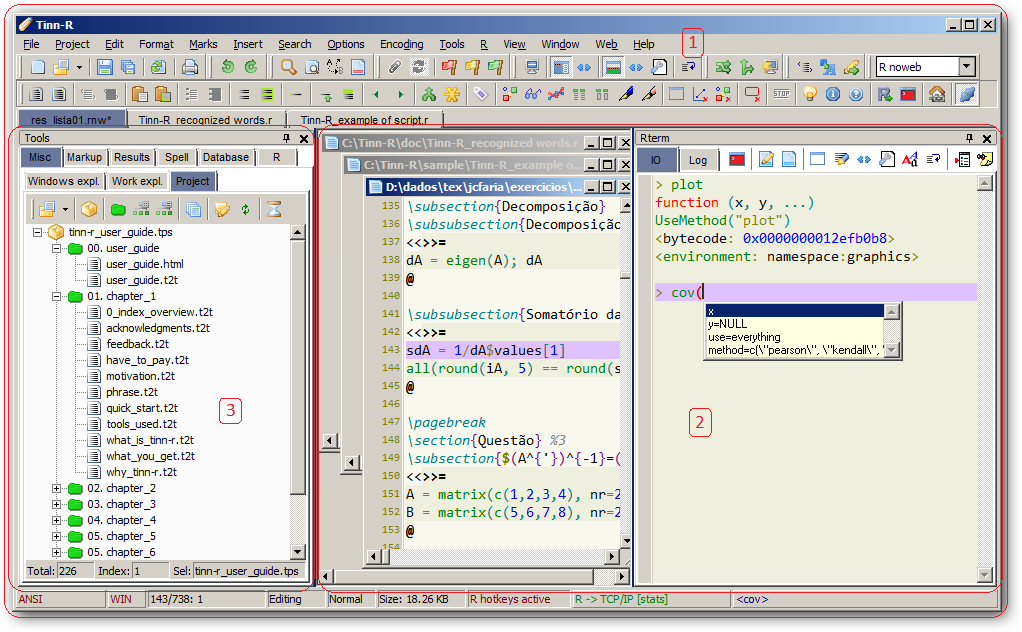
\includegraphics[width=\headwidth]{./res/parts_01.png}
  \end{center}
  \caption{Tinn-R: Main resources.}
  \label{fig:tinn-r_interface}
\end{figure}

Tinn-R interface
(Figure \ref{fig:tinn-r_interface})
is very flexible and user configurable. It is necessary time
to know all available resources and to configure this out (according to your
preferences) in a nice way. The default set of options might not be suitable
for every user.

The window \textit{Application options} allows the user to set the major piece
of user preferences related to the application.

It must be clear from now on that the Tinn-R project is the sum of three main
resources (Figure \ref{fig:tinn-r_interface}):
The application \texttt{per se (1)},
the instances of the \texttt{SynEdit class (2)}
and additional \texttt{Tools (3)},
the latest one projected to allows the expansion of resources.
\index{application options}

The options visible in all pictures reflect a set of the project coordinator
preferences.


\hypertarget{working_app_main}{}
\subsection{Main}
\index{application options!main}

\begin{figure}[h!]
  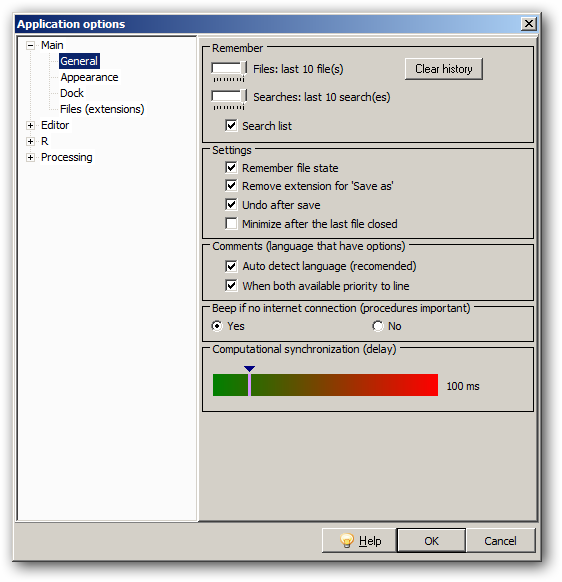
\includegraphics[scale=0.35]{./res/app_main_general.png}~~
  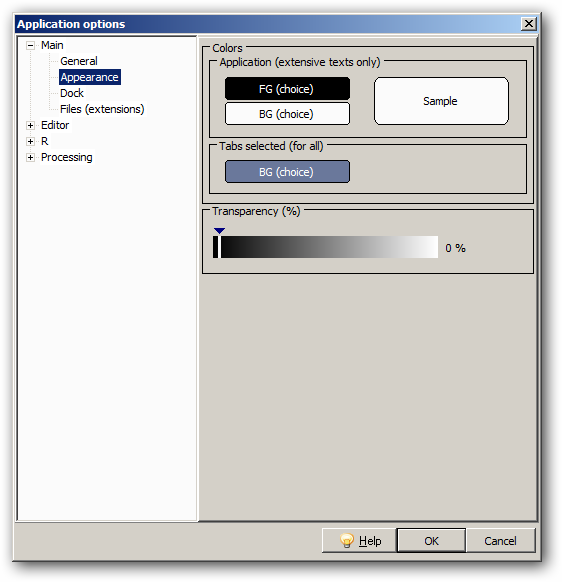
\includegraphics[scale=0.35]{./res/app_main_appearance.png}\\
  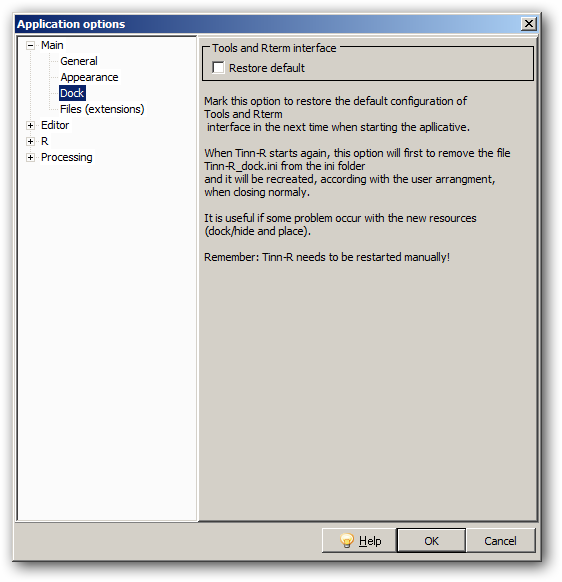
\includegraphics[scale=0.35]{./res/app_main_dock.png}~~
  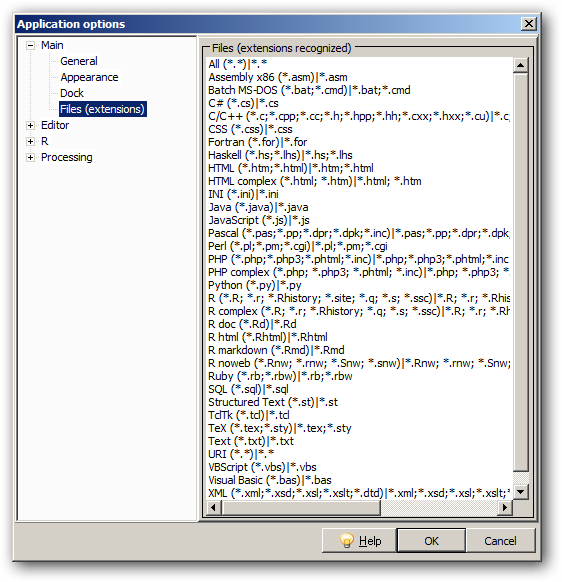
\includegraphics[scale=0.35]{./res/app_main_files.png}\\
  \caption{Main (Options/Application).}
  \label{fig:app_main_options}
\end{figure}

\begin{table}
  \begin{footnotesize}
    \begin{tabularx}{\headwidth}{>{\hsize=0.35\hsize}X>{\hsize=0.65\hsize}X}\\
      \hline
      \textbf{Option} & \textbf{Description} \\
      \hline
      Computational syncronization (delay) & Several processes are dependent on synchronization between applications
       (\RR{}, converters, compilers). The optimal value of the delay is determined by the following characteristics:
       user habits, hardware and software available.
       The ideal value is unique to the various possible combinations of those three characteristics.
       Try to reduce to the minimum value (50 ms) and test it: if something does not work, increase it gradually
       and keep testing until getting to the optimal value. The default value (100 ms) may not be optimal for all users. \\
      Remove extension for \textit{Save as} & All file extensions will be removed
       in the \textit{Save as} Windows interface \\
      Application colors (extensive text only) & Dark colors (low level of radiation)
       for the background, and pale light (high level of radiation) for the characters
       are reccomended for people who work with the computer/monitor for long periods.
       Pictures of this user guide ire like this \\
      \hline
    \end{tabularx}
  \end{footnotesize}
  \caption{Same main options}
  \label{tab:app_main}
\end{table}

Figure \ref{fig:app_main_options} and
Table \ref{tab:app_main}
show the options related to this topic.

Since the options are self-explanatory, Table \ref{tab:app_main} only gives some
details about the most difficult options to understand.


\hypertarget{working_app_r}{}
\subsection{R}
\index{application options!R}

\begin{figure}[h!]
  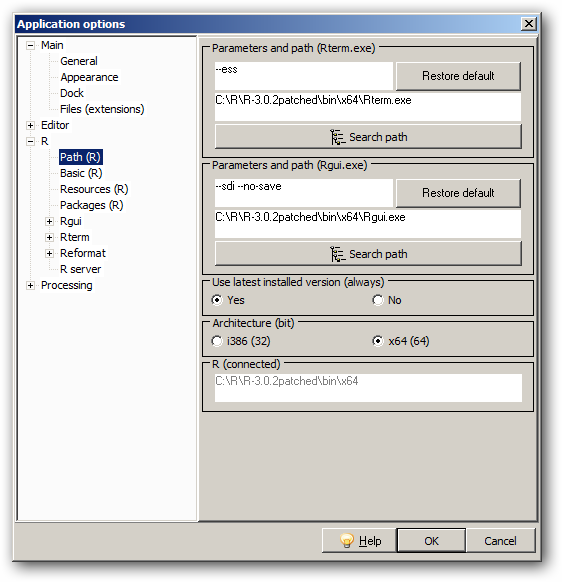
\includegraphics[scale=0.35]{./res/app_r_path.png}~~
  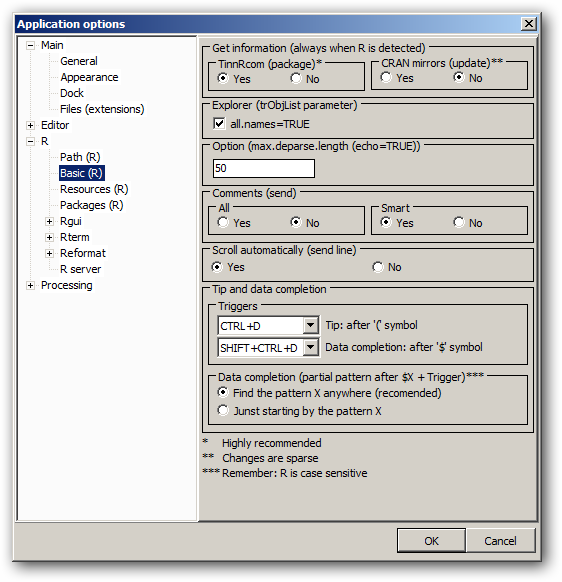
\includegraphics[scale=0.35]{./res/app_r_basic.png}\\
  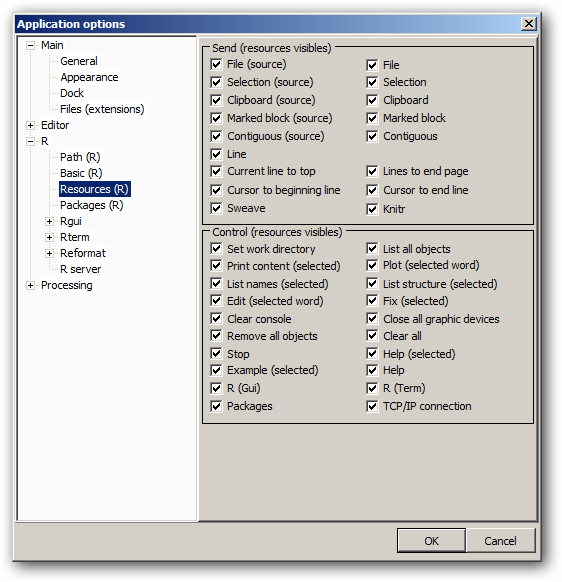
\includegraphics[scale=0.35]{./res/app_r_resources.png}~~
  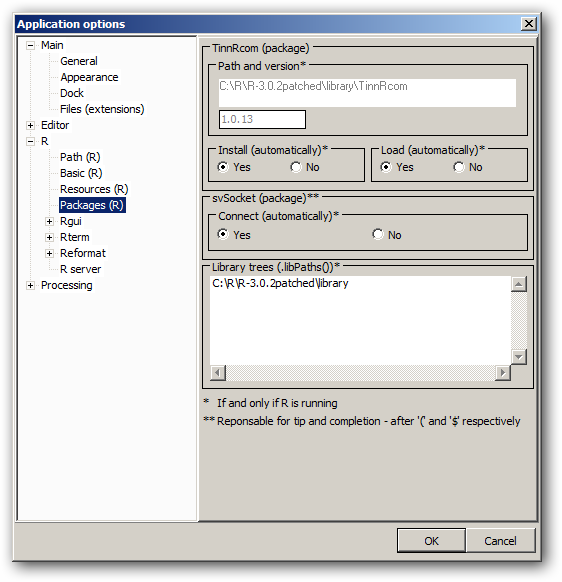
\includegraphics[scale=0.35]{./res/app_r_packages.png}\\
  \caption{R (Options/Application).}
  \label{fig:app_r_a}
\end{figure}

\begin{figure}[h!]
  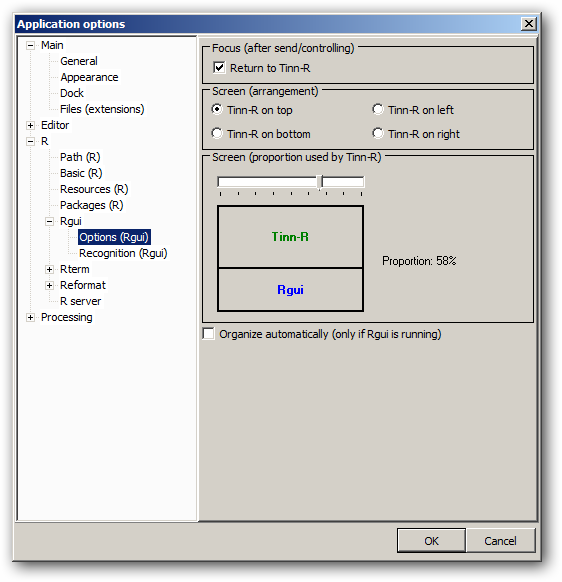
\includegraphics[scale=0.35]{./res/app_r_rgui_options.png}~~
  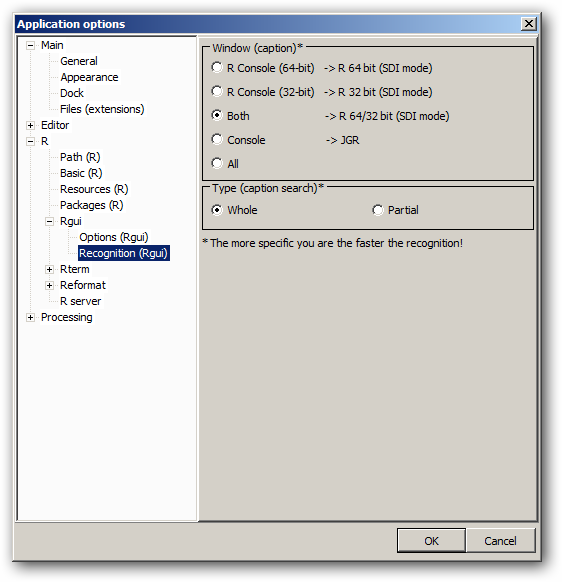
\includegraphics[scale=0.35]{./res/app_r_rgui_recognition.png}\\
  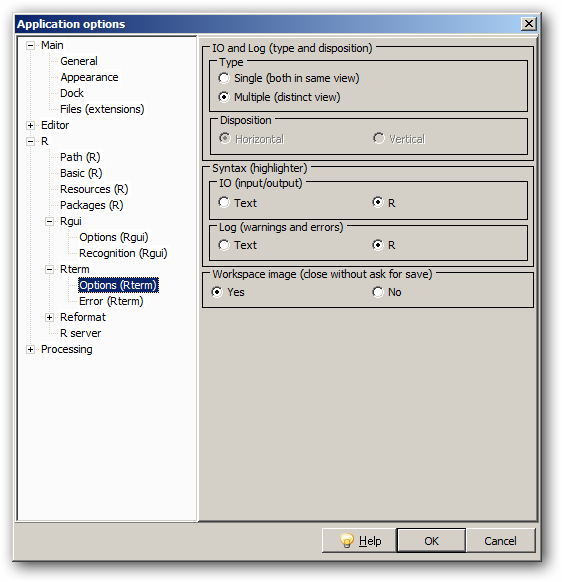
\includegraphics[scale=0.35]{./res/app_r_rterm_options.png}~~
  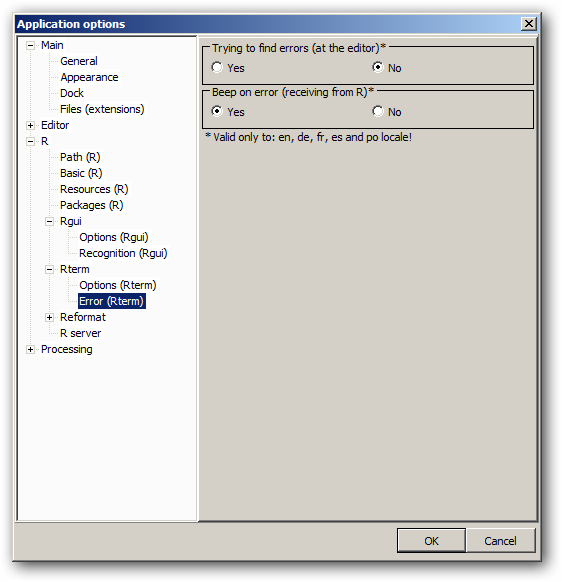
\includegraphics[scale=0.35]{./res/app_r_rterm_error.png}\\
  \caption{R (Options/Application).}
  \label{fig:app_r_b}
\end{figure}

\begin{figure}[h!]
  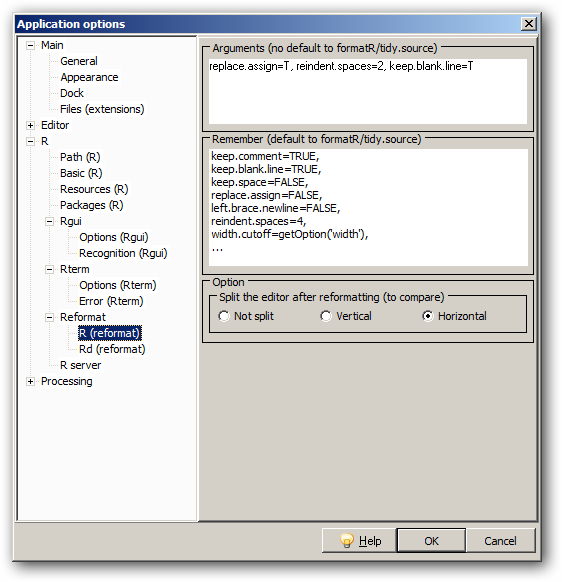
\includegraphics[scale=0.33]{./res/app_r_reformat_r.png}~~
  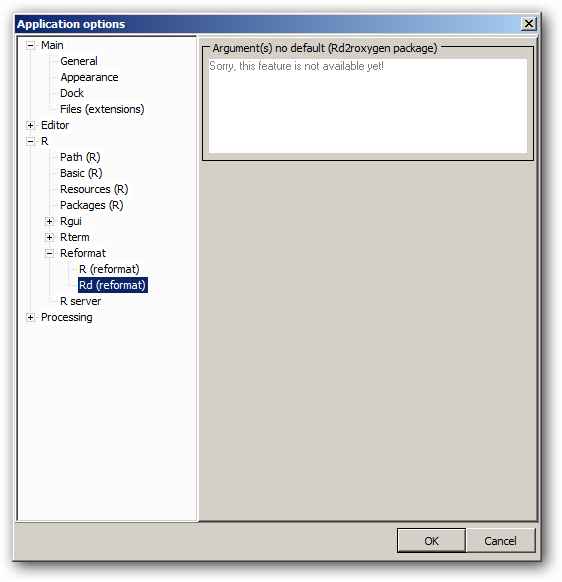
\includegraphics[scale=0.33]{./res/app_r_reformat_rd.png}~~
  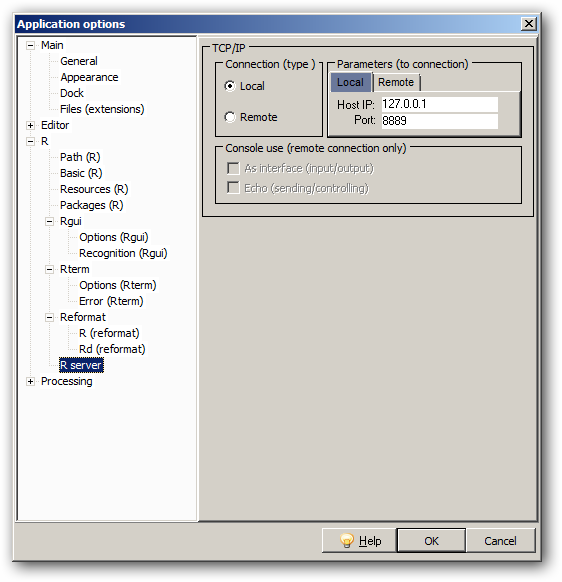
\includegraphics[scale=0.33]{./res/app_r_server.png}\\
  \caption{R (Options/Application).}
  \label{fig:app_r_c}
\end{figure}

Figures \ref{fig:app_r_a}, \ref{fig:app_r_b} and \ref{fig:app_r_c}
shows a set of options available. As you can see, it allows a high level
of customization with the \RR{} environment.


\hypertarget{working_app_processing}{}
\subsection{Processing}
\index{application options!processing}

\begin{figure}[h!]
  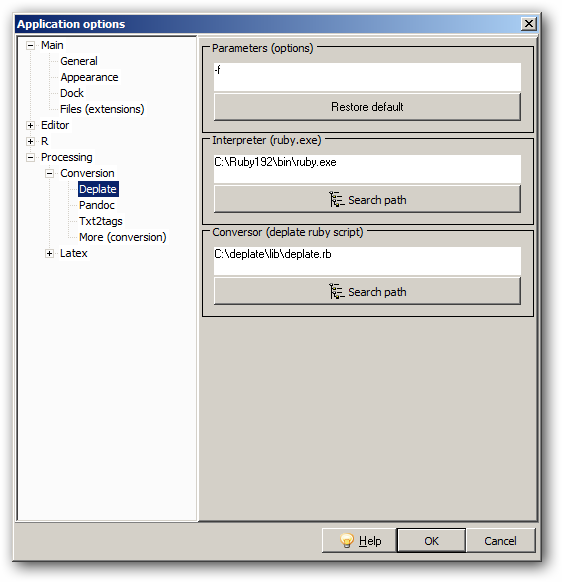
\includegraphics[scale=0.35]{./res/app_processing_conversion_deplate.png}~~
  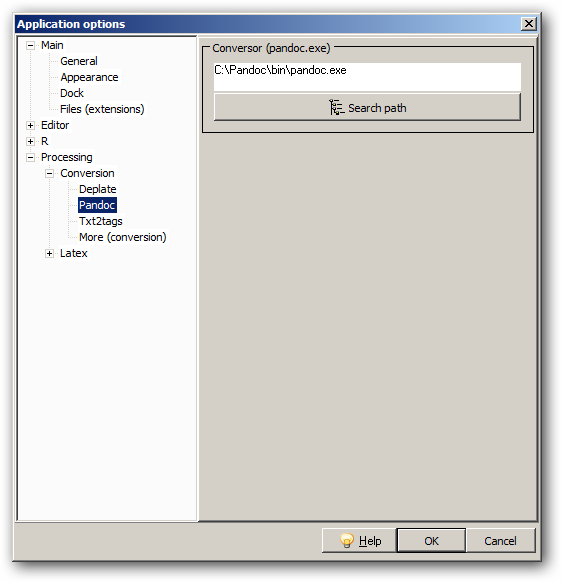
\includegraphics[scale=0.35]{./res/app_processing_conversion_pandoc.png}\\
  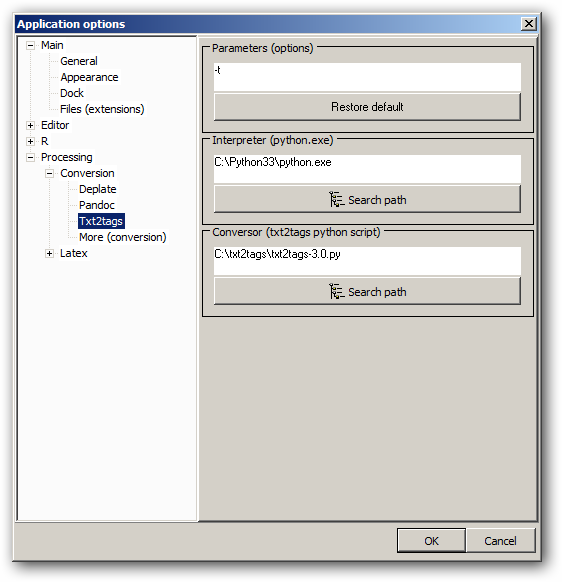
\includegraphics[scale=0.35]{./res/app_processing_conversion_txt2tags.png}~~
  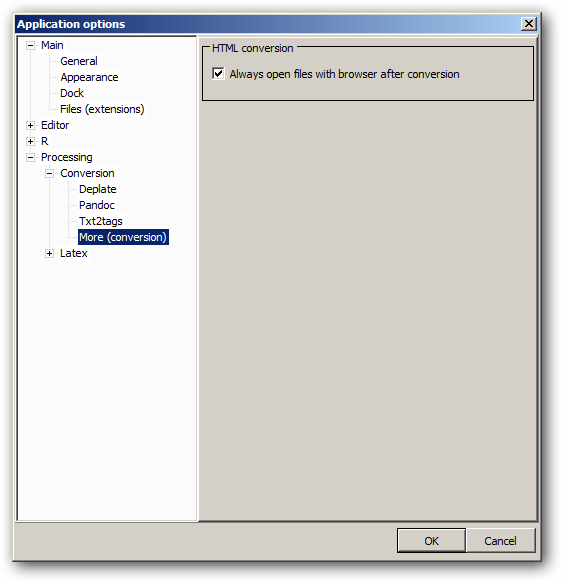
\includegraphics[scale=0.35]{./res/app_processing_conversion_more.png}\\
  \caption{Conversion (Options/Application/Processing).}
  \label{fig:app_processing_conversion_options}
\end{figure}

There are resources
(Figure \ref{fig:app_processing_conversion_options} and
\ref{fig:app_processing_latex_options})
related to conversion (Deplate, Pandoc and Txt2tags) and compilation (Miktex).


\hypertarget{working_app_processing_conversion}{}
\subsubsection{Conversion:}
\index{application options!processing conversion}

Tinn-R project makes it easy to work with these nice conversion tools: Deplate, Pandoc and Txt2tags.
(Figure \ref{fig:app_processing_conversion_options}).


\newpage
\hypertarget{working_app_processing_latex}{}
\subsubsection{LaTex:}
\index{application options!processing LaTeX}

\begin{figure}[h!]
  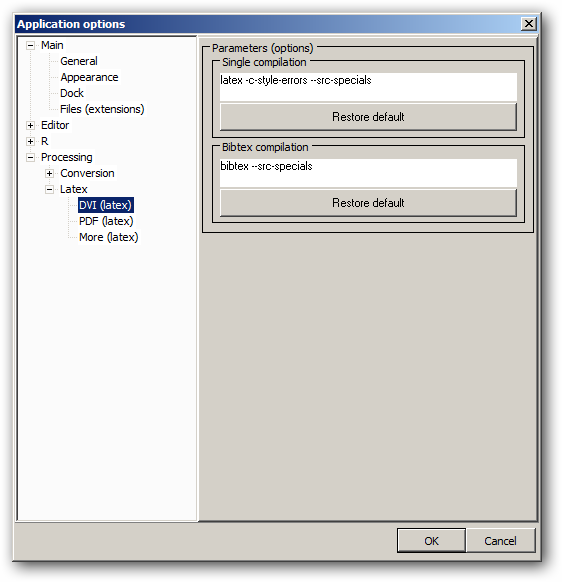
\includegraphics[scale=0.33]{./res/app_processing_latex_dvi.png}~~
  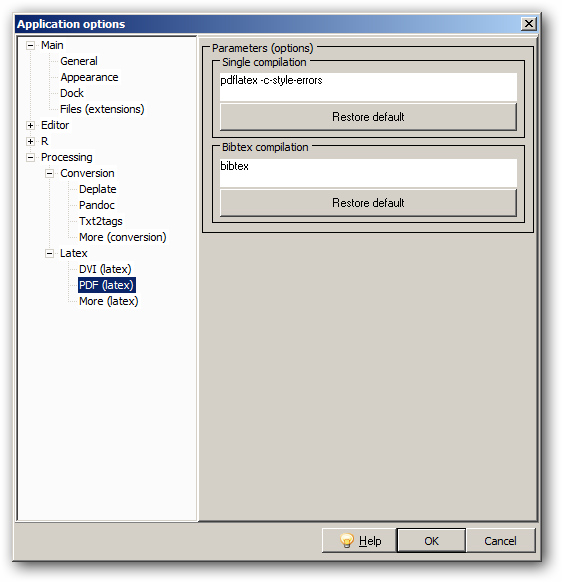
\includegraphics[scale=0.33]{./res/app_processing_latex_pdf.png}~~
  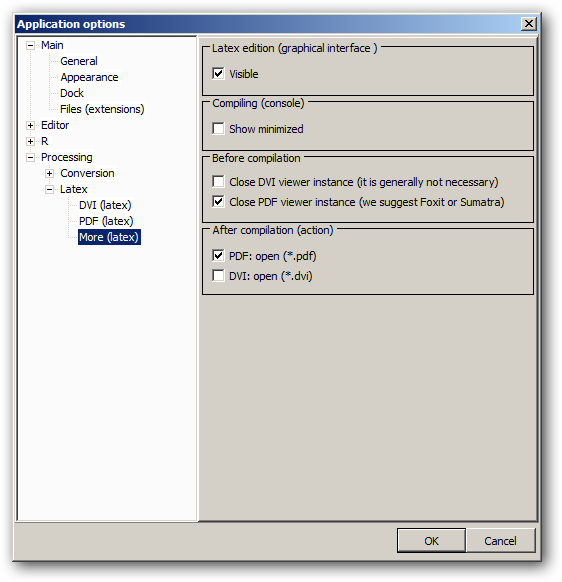
\includegraphics[scale=0.33]{./res/app_processing_latex_more.png}\\
  \caption{Latex (Options/Application/Processing).}
  \label{fig:app_processing_latex_options}
\end{figure}

Tinn-R is not a specific editor to \LaTeX, but it has the basic resources (Figure \ref{fig:app_processing_latex_options}) allowing the user to use the main resources of this environment.
